{\huge Max Bahr online}\\



Zwei Wochen ist es nun her, dass die Menschen aus der Zeltstadt am Polizeipräsidium Osthessen in den ehemaligen Baumarkt von Max Bahr umgezogen sind. Die Zeltstadt wurde seit Mitte September von der Fuldaer Freifunk Community mit freiem Wlan und damit auch mit Internet versorgt. Dies wollten wir nun auch im Max Bahr ermöglichen.\\

Der neue Standort der Flüchtlingsunterkunft stellte uns vor die Herausforderung, zunächst einmal eine Anbindung an unser bestehendes Netz in Fulda zu realisieren. Glücklicherweise fand sich ein Bürger, der seine Internetverbindung zur Verfügung stellt und der auch noch eine perfekte Sichtverbindung zum alten Baumarkt hat. Also ging es an die Planung, wie man eine Richtfunkstrecke zur Versorgung aufbauen kann.\\

Heute Nachmittag war nun ein Außenteam vor Ort und hat 6 Router, einen Accesspoint und die Gegenstelle der Richtfunkstrecke aufgebaut. Seit ca. 19:30 Uhr haben wir unsere neuen Knoten auf dem Meshviewer.\\

Der Aufbau gestaltete sich vor allem deswegen schwierig, weil wir keinen direkten Zugang zu Dach finden konnten. Selbst mit Hilfe des Facility-Managements war kein herkömmlicher Weg nach oben zu finden, also mussten wir uns eine Leiter organisieren und dann konnte eine Nano-Station aufgebaut werden, welche per Netzwerkkabel mit Strom aus dem Erdgeschoss versorgt wird. Die Wartezeit überbrückten wir mit dem Aufhängen der 6 Router, die dann das Wlan für die Flüchtlinge bereit stellen. Zunächst noch mit fragenden Blicken bedacht wurden wir schnell als diejenigen identifiziert, die das WIFI installieren. \\

Schon kurz nach Aktivierung waren dann auch schon bis zu 50 Clients eingeloggt. Alles in allem ein aufregender und toller Nachmittag. \\

% \begin{center}
\vspace{1.3cm}
\hspace{1.4cm}
\scalebox{0.80}{
\begin{row}{3}{2}
  \noindent%
  \begin{cell}{2}
   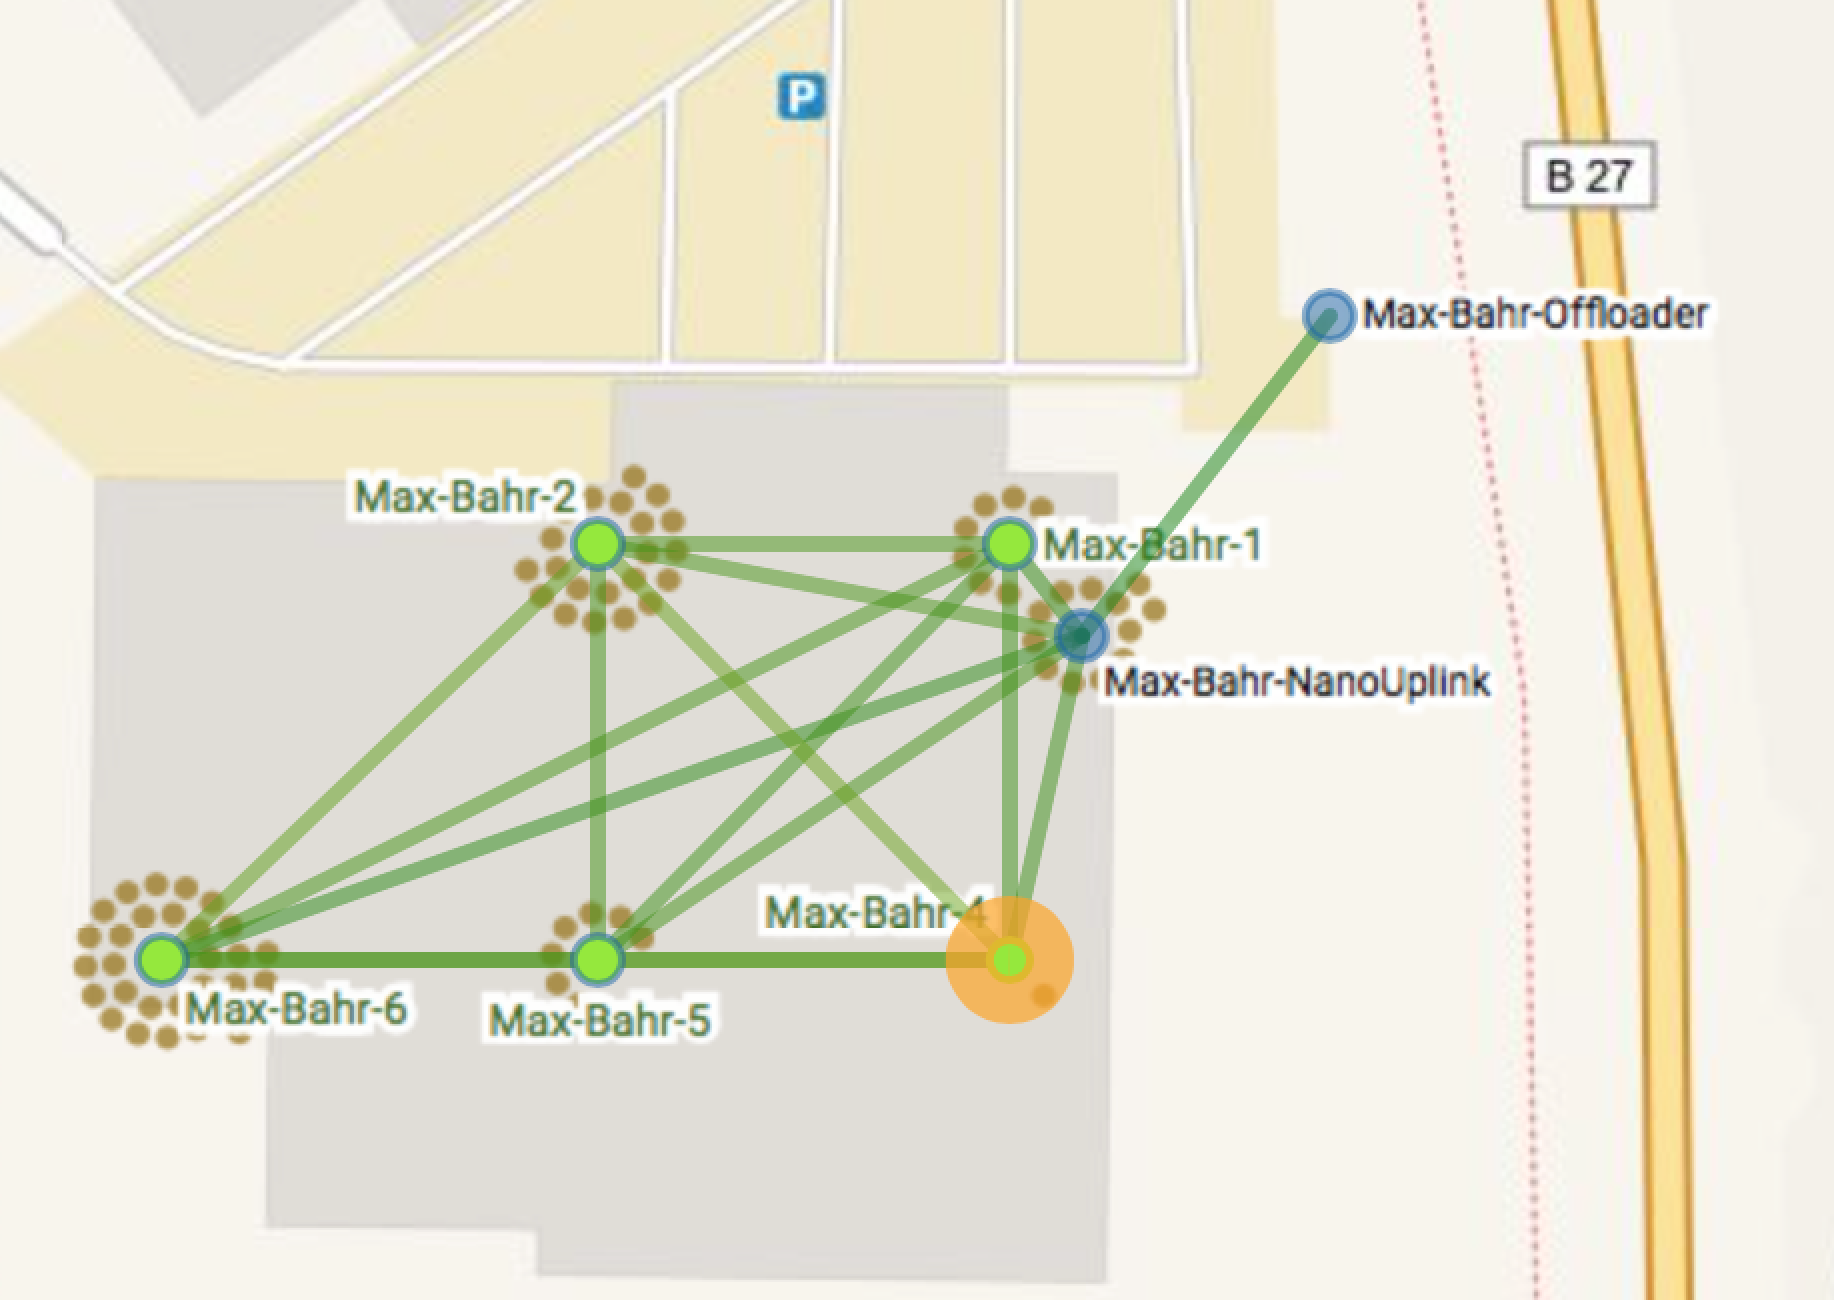
\includegraphics[height=110mm,width=110mm]{./MaxBahrMesh.png}
  \end{cell}
  \begin{cell}{1}
  \vspace{-8.5cm}
   \includegraphics[height=55mm,width=55mm]{./statistik.png}
  \end{cell}
\end{row}
}
% \end{center}



\newpage
\begin{textblock*}{190mm}(10mm,10mm)
\includegraphics[height=190mm,width=190mm]{./maxbahrPlanungQuad.png}\\
% \color{white}
\end{textblock*}

Da es im ehemaligen Max Bahr keinen Zugang zu Flachdach gibt,\\
war es nötig über Leitern auf das Dach zu kommen.\\
In der Grafig sieht man die Standorte der Freifunk-Router \\
und die Lage der Wohnbereiche.\\
 




 \newpage
 \begin{textblock*}{40mm}(15mm,35mm)
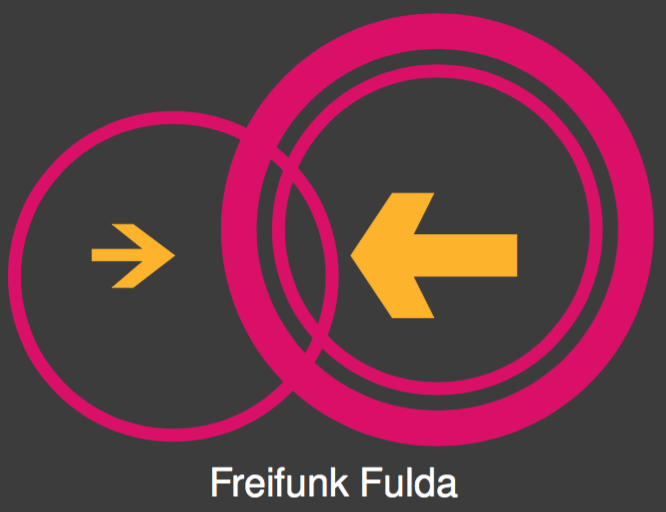
\includegraphics[height=30mm,width=39mm]{./FFLogo.png}\\
% \color{white}
\end{textblock*}

 \begin{textblock*}{190mm}(10mm,60mm)
\includegraphics[height=190mm,width=190mm]{./Uplink_Kabel.png}\\
% \color{white}
\end{textblock*}
 \begin{textblock*}{190mm}(90mm,35mm)
Die Richtfunkstrecke wurde mit 2 Ubiquiti Nano Stations realisiert.\\
Das sind Wlan-Acces-Points für den Außeneinsatz mit integrierter \\Richtantenne.\\
Da diese Geräte ihren benötigten Strom über das Netzwerkkabel\\
erhalten, musste somit nur ein Kabel von der Nano Station zum \\
ersten Freifunk-Router (Max-Bahr-NanoUplink) gelegt werden.

\end{textblock*}
















